\subsubsection[多变量函数的连续性]{Continuity}

\begin{definition}
    Let $f:\,D\left(\subseteq\mathbb{R}^2\right)\to\mathbb{R}$ and $M_0\in D$, we say $f$ is continuous at $M_0$ if $\lim_{M\to M_0}f(M)=f(M_0)$, i.e. $\forall\varepsilon>0$, $\exists\delta=\delta(\varepsilon)>0$ s.t. $\forall M\in D\cap B\left(M_0,\delta\right)$, $\left|f(M)-f\left(M_0\right)\right|<\varepsilon$
\end{definition}

\begin{example}
    $D=\left\{(x,y)\in\mathbb{R}^2\mid xy>-1\right\}$, $f(x,y)=\begin{cases}
            \log(1+xy)^{\frac{1}{xy}} & xy\neq 0 \\
            1                         & xy=0
        \end{cases}$

    $\forall\varepsilon>0$, $\exists\delta=\delta(\varepsilon)>0$, $\forall\left|u-x_0y_0\right|<\delta$

    \allbold{Need $\left|xy-x_0y_0\right|<\delta\implies\left|f(x,y)-f\left(x_0,y_0\right)\right|<\varepsilon$\\
        $\left|xy-x_0y_0\right|=\left|x_0\right|\left|y-y_0\right|-|y|\left|x-x_0\right|$}
    {\boldmath\begin{align*}
            \left(\left|x_0\right|+2\left|y_0\right|+1\right)\left(\left|x-x_0\right|+\left|y-y_0\right|\right) & \geq\left|x_0\right|\left|y-y_0\right|-|y|\left|x-x_0\right| \\
                                                                                                                & \geq\left|x_0y-x_0y_0\right|+\left|xy-x_0y\right|            \\
                                                                                                                & \geq\left|f(x,y)-f\left(x_0,y_0\right)\right|
        \end{align*}}

    \begin{center}
        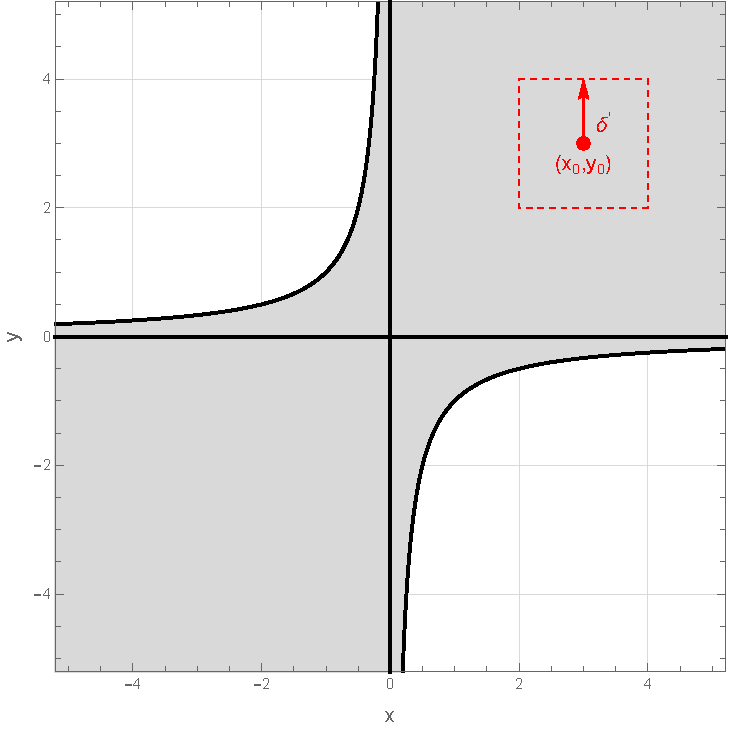
\includegraphics[height=5cm]{chapters/09/01/0401}
    \end{center}

    \allbold{Take $\delta'=\min\left\{\frac{\delta}{2\left(\left|x_0\right|+2\left|y_0\right|+1\right)}\left|y_0\right|\right\}$.}

    \allbold{Then $\forall\left|x-x_0\right|<\delta'$, $\left|y-y_0\right|<\delta'$, $\left|xy-x_0y_0\right|<\delta'$, $\left|f(x,y)-f\left(x_0,y_0\right)\right|<\varepsilon$}
\end{example}

\begin{example}[Angle Function]
    \raisebox{-0.5\height}{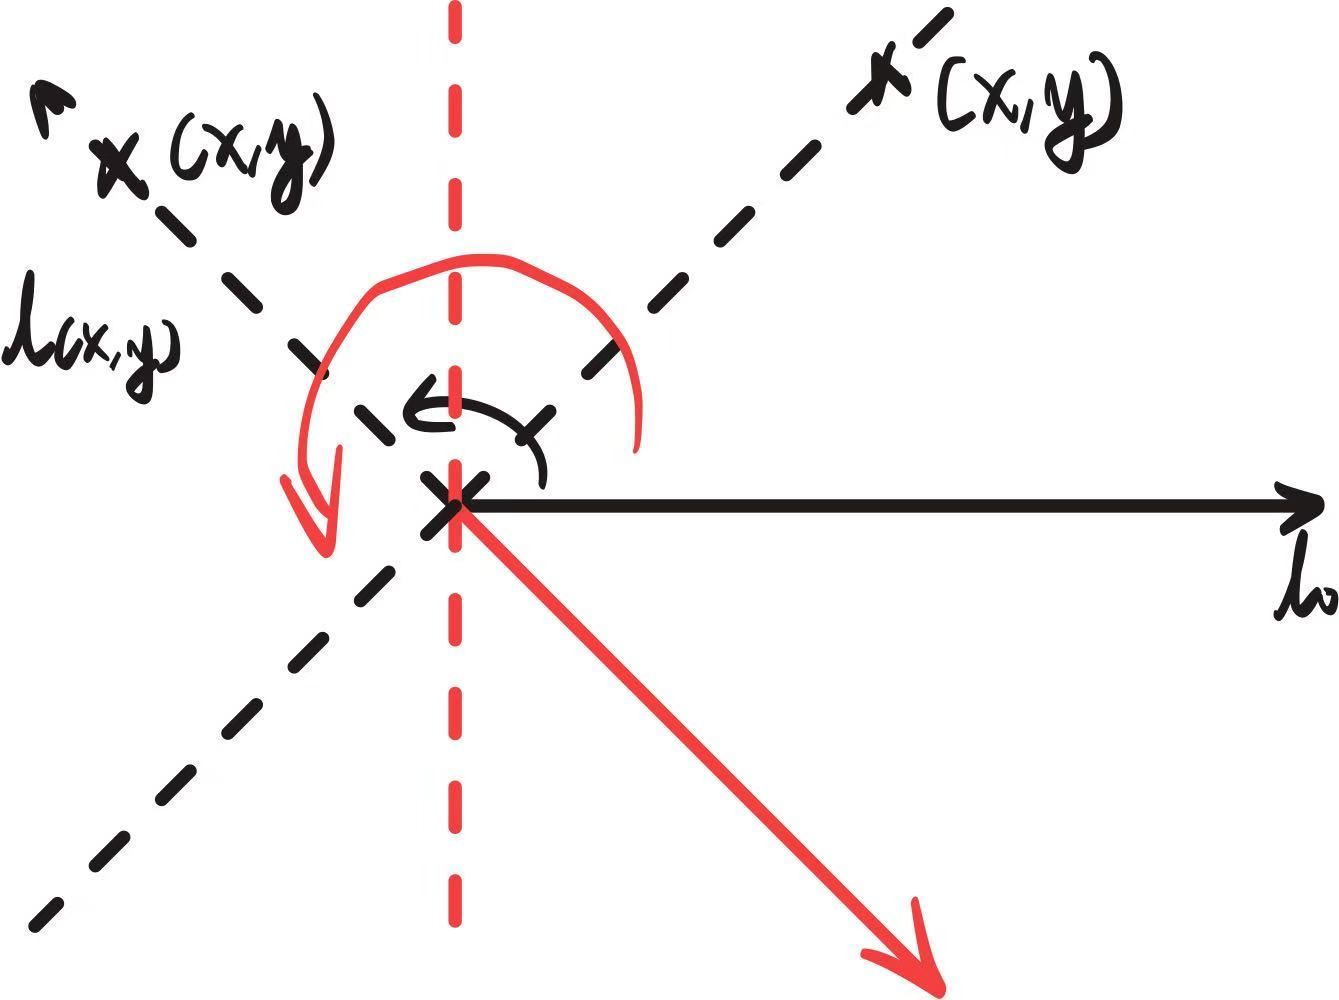
\includegraphics[height=2cm]{chapters/09/01/0402}}

    $\begin{cases}
            r=\sqrt{x^2+y^2} \\
            \theta=\text{the angle between the ray $l_0$ and $l_{(x,y)}$ counted anti-clockwised}
        \end{cases}$\\\allbold{$(x,y)\in\mathbb{R}^2\setminus\left\{(0,0)\right\}$}

    $$=\begin{cases}
            \arctan\frac{y}{x}      & x>0,\,y>0 \\
            \frac{\pi}{2}           & x=0,\,y=0 \\
            \pi+\arctan\frac{y}{x}  & x<0       \\
            \frac{3\pi}{2}          & x=0,\,y<0 \\
            2\pi+\arctan\frac{y}{x} & x>0,\,y<0
        \end{cases}$$

    $\tan:\,\left(-\frac{\pi}{2},\frac{\pi}{2}\right)\xrightarrow{\text{1:1}}\mathbb{R}$

    $\xrightarrow{\text{inverse}}\arctan:\,\mathbb{R}\to\left(-\frac{\pi}{2},\frac{\pi}{2}\right)$

    \textbf{Conclusion}:\begin{enumerate}
        \item $\theta$ is continuous on $\mathbb{R}^2\setminus[0,+\infty)$ but has jumping discontinuity on $(0,+\infty)$
        \item $r$ is continuous on $\mathbb{R}^2$
    \end{enumerate}
\end{example}

\begin{definition}[Uniform Continuity]
    Let $f$ be defined on $D\subseteq\mathbb{R}^2$, $f$ is said to be uniformly continuous if $\forall\varepsilon>0$, $\exists\delta=\delta(\varepsilon)>0$, s.t. $\forall M',M''\in D$, $d\left(M',M''\right)<\delta$, $\left|f\left(M'\right)-f\left(M''\right)\right|<\varepsilon$
\end{definition}

\begin{theorem}
    \begin{enumerate}
        \item The continuity of function is preserved under $+,-,\times$ and $\div$ (provided the denominator function is nonzero at the point of interest)
        \item The composition of continuous vector-valued functions is continuous.
        \item \emph{(Intermediate Value Property)} Let $f$ be defined on a \emph{connected} set $D\subseteq\mathbb{R}^2$, and $f$ is continuous. Then for any $M_1,M_2\in D$, all values between $f\left(M_1\right)$ and $f\left(M_2\right)$ can be achieved. \emph{In particular, $f(D)$ is an interval.} (More generally, the image of a connected set under a continuous vector-valued function is connected.)
              \begin{pf}
                  Argue by contradiction.

                  Suppose $f(D)$ is not connected. Then $f(D)=A\sqcup B$, $A,B\neq\emptyset$, $A\cap\overrightarrow{B}=\emptyset$, $B\cap\overline{A}=\emptyset$.

                  $\implies D=f^{-1}(A)\sqcup f^{-1}(B)$, $f^{-1}(A),f^{-1}(B)\neq\emptyset$

                  \emph{Suppose $\left\{M_n\right\}\subseteq f^{-1}(A)$}, $M_n\to M_0\in f^{-1}(B)$, then $\overset{\substack{A\\\downarrow}}{f\left(M_n\right)}\to\overset{\substack{B\\\downarrow}}{f\left(M_0\right)}\implies B\cap\overline{A}\neq\emptyset$, contradiction.

                  $\implies\overline{f^{-1}(A)}\cap f^{-1}(B)=\emptyset$

                  Similarly, $\implies\overline{f^{-1}(B)}\cap f^{-1}(A)=\emptyset$

                  $\implies$ This is a contradiction with the connectivity of $D$.
              \end{pf}
        \item The $\overset{\substack{\text{\textbf{supremum}}\\\uparrow}}{\text{\emph{maximum}}}$ and $\overset{\substack{\text{\textbf{infimum}}\\\uparrow}}{\text{\emph{minimum}}}$ of a continuous function on a bounded closed set can be achieved.
              \begin{pf}
                  \emph{Step 1)\quad}$\sup_Df<+\infty$, $\inf_Df>-\infty$

                  If $\sup_Df=+\infty$, then $\exists\left\{M_n\right\}\subseteq\overset{\substack{\text{closed, bounded}\\\downarrow}}{D}$, s.t. $f\left(M_n\right)\to+\infty$

                  By Bolzano-Weierstrass Thm, $\exists$ subsequence $\left\{M_{n_k}\right\}$ s.t. $M_{n_k}\to M_0\in D\,(k\to+\infty)$, $f\left(M_{n_k}\right)\to f\left(M_0\right)=+\infty\,(k\to+\infty)$ by continuity, contradiction.

                  \emph{Step 2)\quad}$\sup_Df=f\left(M_0\right)$ for some $M_0\in D$

                  Suppose $\sup_Df\neq f(M)$ for any $M\in D$

                  \begin{align*}
                       & \implies\exists\left\{M_n\right\}\subseteq D\text{ s.t. }f\left(M_0\right)\to\sup_Df                                                                                         \\
                       & \overset{\text{B.W.}}{\implies}\exists\text{ subsequence }\left\{M_{n_k}\right\}\subseteq D,\,M_{n_k}\to M_0\in D\implies f\left(M_{n_k}\right)\to f\left(M_0\right)=\sup_Df
                  \end{align*}
              \end{pf}
        \item \emph{(Cantor Thm)} Continuous function on a bounded closed set is uniformly continuous.
    \end{enumerate}
\end{theorem}